%%%%%%%%%%%%%%%%%%%%%%%%%%%%%%%%%
\chapter{クイーン支配問題の制約モデル}\label{chap:constraint}
%%%%%%%%%%%%%%%%%%%%%%%%%%%%%%%%%
本章では,提案する基本制約モデル,改良制約モデル,部分和制約モデル
についての説明を行う.
各制約モデルにおいて,
入力はクイーングラフ$Q_{n}$と正の整数$k$である.

\section{基本制約モデル}
\begin{description}
 \item[(変数$q_{ij}$)] $q_{ij} \in \{0,1\}$ \par
1のとき,マス$(i,j)$にクイーンが配置されることを意味する.
 \item[(制約1)] $\sum\limits_{i,j=1}^{n} q_{ij} = k$ \par
クイーングラフ上のクイーンの総数が$k$であることを意味する.
 \item[(制約2)] $(\bigvee\limits_{(i',j')\in A_{ij}} 
q_{i'j'}) >0 \qquad (1 \leq i,j \leq n)$ \par
マス$(i,j)$に1つ以上のクイーンが移動できることを意味する.
ここで,$A_{ij}$はマス$(i,j)$にクイーンが移動できるマスの集合を表す.
\end{description}

このモデルを$n=3,k=2$で実行すると,コード~\ref{code:3-2_model0}のように
変数と節が生成される.なお,コード~\ref{code:3-2_model0}において,
\code{(int }  \code{q_i_j }  \code{0  1)}は\code{q_i_j}が
0または1の値を取る変数であること,\code{(= (+ q_1_1 } \code{... } 
\code{q_3_3) 2)}は\code{(q_1_1 } \code{+ ... + } 
\code{q_3_3 = 2)}であること,\code{(> (+ q_1_1 } \code{... } 
\code{q_3_3) 0)}は\code{((q_1_1 } \code{+ ... + } 
\code{q_3_3) > 0)}であることを表す.

生成された節に着目すると,(制約2)で生成される節において,
例えば16-18行目の\code{(+ q_1_1 q_1_2 q_1_3 ...)}のように
同じ部分式が複数の節で出現していることがわかる.
\lstinputlisting[float=ht,caption={%
基本制約モデルの実行例($n=3,k=2$)},%
captionpos=b,frame=single,label=code:3-2_model0,%
numbers=none,%
breaklines=true,%
columns=fullflexible,keepspaces=true,%
basicstyle=\ttfamily\scriptsize]{code/qdp_3-2_model0.log}

\newpage
\section{改良制約モデル}
本モデルでは,基本制約モデルにおいて複数回出現する部分式を
まとめるための補助ブール変数と制約を追加する.

各行に対して以下の補助ブール変数と制約を追加する.
\begin{description}
 \item[(変数$r_i$)] $r_{i} \in \{0,1\} \qquad (1 \leq i \leq n)$\par
  1のとき,行$i$にクイーンが1つ以上存在することを意味する.
 \item[(制約3)] $r_{i}>0 \rightarrow \bigvee\limits_{(i',j')\in R_{i}} q_{i'j'}=1 \qquad (1 \leq i \leq n)$ \par
  $r_{i}$が1のとき,行$i$上にクイーンが1つ以上配置されていることを意味する.
  ここで,$R_i$は行$i$上に存在する頂点の集合を表す.
\end{description}
%
各列,各右上がり対角線,各右下がり対角線についても同様に,
補助ブール変数$c_{j}$,$u_{a}$,$d_{b}$を追加し,
(制約4),(制約5),(制約6)を追加する.
%
\begin{description}
 \item[(制約4)] $c_{j}>0 \rightarrow \bigvee\limits_{(i',j')\in C_{j}} q_{i'j'}=1 \qquad (1 \leq j \leq n)$ 
 \item[(制約5)] $u_{a}>0 \rightarrow \bigvee\limits_{(i',j')\in U_{a}} q_{i'j'}=1 \qquad (1 \leq a \leq 2n-1)$ 
 \item[(制約6)] $d_{b}>0 \rightarrow \bigvee\limits_{(i',j')\in D_{b}} q_{i'j'}=1 \qquad (1 \leq b \leq 2n-1)$ \par
  ここで,$C_j$,$U_{a}$,$D_{b}$はそれぞれ列$j$,右上がり対角線$a$,
  右下がり対角線$b$上に存在する頂点の集合を表す.
\end{description}

さらに,基本制約モデルの(制約2)を削除し,以下の(制約7)に置き換える.
\begin{description}
 \item[(制約7)] $(r_i > 0) \vee (c_j >0) \vee (u_{a}>0) \vee (d_{b}>0) \qquad (1 \leq i,j \leq n)$
\end{description}

このモデルを$n=3,k=2$で実行すると,コード~\ref{code:3-2_model1}のように
変数と節が生成される.なお,コード~\ref{code:3-2_model1}において,
\code{(imp (> r_1 0) }\code{(> (+ q_1_1 } \code{q_1_2 } 
\code{q_1_3) 0))}は\code{((r_1 > 0)} $\rightarrow$ 
\code{(q_1_1 } \code{+ q_1_2 } \code{+ q_1_3 } 
\code{> 0))}であること,\code{(or (> r_1 0) } \code{(> c_1 0) } 
\code{(> u_1 0)} \code{(> d_3 0))}は\code{(r_1 > 0} $\vee$ 
\code{c_1 > 0} $\vee$ \code{u_1 > 0} $\vee$ \code{d_1 > 0)}を表す.
\lstinputlisting[float=ht,caption={%
改良制約モデルの実行例($n=3,k=2$)},%
captionpos=b,frame=single,label=code:3-2_model1,%
numbers=none,%
breaklines=true,%
columns=fullflexible,keepspaces=true,%
basicstyle=\ttfamily\scriptsize]{code/qdp_3-2_model1.log}


\newpage
\section{部分和制約モデル}
本モデルでは,クイーンの個数を表す補助整数変数を追加し,
行方向,列方向,対角線方向のクイーンの総数に関する制約を追加する.
\begin{description}
 \item[(変数$r_i$)] $r_{i} \in \{0,...,k\}$ 
 \item[(制約8)] $r_{i} = \sum\limits _{(i',j') \in R_{i}} q_{i'j'} \qquad (1 \leq i \leq n)$ \par
$r_i = s$のとき,行$i$にクイーンが$s$個存在することを意味する.
\end{description}
%
各列,各右上がり対角線,各右下がり対角線に対しても同様に
補助整数変数$c_j$,$u_{a}$,$d_{b}$と(制約9),(制約10),(制約11)を追加する.
%
\begin{description}
 \item[(制約9)] $c_{j} = \sum\limits _{(i',j') \in C_{j}} 
q_{i'j'} \qquad (1 \leq i \leq n)$
 \item[(制約10)] $u_{a} = \sum\limits _{(i',j') \in U_{a}} 
q_{i'j'}\qquad (1 \leq a \leq 2n-1)$
 \item[(制約11)] $d_{b} = \sum\limits _{(i',j') \in D_{b}} 
q_{i'j'} \qquad(1 \leq b \leq 2n-1)$
\end{description}
さらに,クイーンの総数に関する制約である(制約12)を追加する.
\begin{description}
 \item[(制約12)] $\sum\limits_{i=1}^{n} 
r_{i} = \sum\limits_{j=1}^{n} 
c_{j} =\sum\limits_{a=1}^{2n-1} 
u_{a} =\sum\limits_{b=1}^{2n-1} 
d_{b} = k$ \par
各行,各列,各対角線ごとにクイーンの個数を足し合わせると
クイーンの総数$k$に等しいことを意味する.\par

部分和制約モデルにより起こる制約伝播を図~\ref{fig:constraint}に示す.
説明のため,上から行1,行2, \dots , 行5とする.
図~\ref{fig:constraint}における$X$と書かれたマスはクイーンが
置かれないと仮定したマスである.まず,図~\ref{fig:constraint}の
赤丸のマスを被覆するために行1にクイーンが置かれなければならない.
同様に,青丸のマスを被覆するために行2に,オレンジ色のマスを被覆するために
行5にクイーンが置かれなければならない.以上から,
$r_1 \geq 1$かつ$r_2 \geq 1$かつ$r_5 \geq 1$である
(図~\ref{fig:constraint}の左の状態).さらに,(制約12)より,
$\sum\limits _{i=1}^{5} r_i = 3$であることから,
$r_1 = 1,r_2=1,r_3=0,r_4=0,r_5=1$であることがわかり,
図~\ref{fig:constraint}の右の図のように制約伝播が起こる.
これにより,探索空間の枝刈りが期待できる.

\begin{figure}[htb]
 \begin{minipage}[b]{0.45\linewidth}
  \centering
  %%%%%%%%%%%%%%%%%%%%%%%%%%%%%%%%%%%%%%%%%%%%%%%%%%
% 実行例(t=0) (第6章で使う)
%%%%%%%%%%%%%%%%%%%%%%%%%%%%%%%%%%%%%%%%%%%%%%%%%%

\begin{tikzpicture}[scale=0.6]

  % 設定
  \tikzset{node/.style={circle,draw=black}}
 
  \definecolor{col_r}{RGB}{230,0,18}
  %\definecolor{col_b}{RGB}{0,104,183}
  \definecolor{col_b}{RGB}{51,51,179}
  \definecolor{col_y}{RGB}{255,251,0}
  \definecolor{col_g}{RGB}{0,96,0}
 
  % 補助線
  % \draw [help lines,blue] (0,0) grid (20,6);
 
  % node %
  \node[node, fill=col_y!70] (node1){\textbf{1}};
  \node[node, fill=col_b!70, right=of node1] (node2){\textbf{2}};
  \node[node, fill=col_y!70, below=of node1] (node3){\textbf{3}};
  \node[node, fill=col_g!70, below=of node2] (node4){\textbf{4}};
 
  \foreach \u / \v in {node1/node2, node2/node3, node2/node4, node3/node4}
  \draw (\u) -- (\v);
 \end{tikzpicture}
 
 %%%%%%%%%%%%%%%%%%%%%%%%%%%%%%%%%%%%%%%%%%%%%%%%%%%%%%%%%%
 %%% Local Variables:
 %%% mode: japanese-latex
 %%% TeX-master: paper.tex
 %%% End:
 
 \end{minipage}
 \begin{minipage}[b]{0.45\linewidth}
  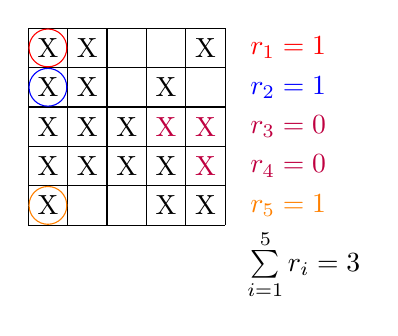
\begin{tikzpicture}
 \draw (0,0)--(2.5,0);
 \draw (0,0.5)--(2.5,0.5);
 \draw (0,1.0)--(2.5,1.0);
 \draw (0,1.5)--(2.5,1.5);
 \draw (0,2.0)--(2.5,2.0);
 \draw (0,2.5)--(2.5,2.5);
 \draw (0,0)--(0,2.5);
 \draw (0.5,0)--(0.5,2.5);
 \draw (1.0,0)--(1.0,2.5);
 \draw (1.5,0)--(1.5,2.5);
 \draw (2.0,0)--(2.0,2.5);
 \draw (2.5,0)--(2.5,2.5);
 \node (X) at (0.25,0.25) {X};
 \draw [orange] (0.25,0.25) circle[radius = 0.24];
 \node (X) at (0.25,0.75) {X};
 \node (X) at (0.25,1.25) {X};
 \node (X) at (0.25,1.75) {X};
 \draw [blue] (0.25,1.75) circle[radius = 0.24];
 \node (X) at (0.25,2.25) {X};
 \draw [red] (0.25,2.25) circle[radius = 0.24];
 \node (X) at (0.75,2.25) {X};
 \node (X) at (0.75,0.75) {X};
 \node (X) at (0.75,1.25) {X};
 \node (X) at (0.75,1.75) {X};
 \node (X) at (1.25,0.75) {X};
 \node (X) at (1.25,1.25) {X};
 \node (X) at (1.75,0.25) {X};
 \node (X) at (1.75,0.75) {X};
 \node (X) at (1.75,1.25) {\color{purple}X};
 \node (X) at (1.75,1.75) {X};
 \node (X) at (2.25,0.25) {X};
 \node (X) at (2.25,0.75) {\color{purple}X};
 \node (X) at (2.25,1.25) {\color{purple}X};
 \node (X) at (2.25,2.25) {X};
 \node (A) at (3.30,2.25) {\color{red}$r_{1} = 1$};
 \node (B) at (3.30,1.75) {\color{blue}$r_{2} = 1$};
 \node (M) at (3.30,1.25) {\color{purple}$r_{3} = 0$};
 \node (M) at (3.30,0.75) {\color{purple}$r_{4} = 0$};
 \node (C) at (3.30,0.25) {\color{orange}$r_{5} = 1$};
 \node (D) at (3.50,-0.50) {$\sum\limits_{i=1}^{5}r_{i}=3$};
\end{tikzpicture}
 \end{minipage}
 \caption{部分和制約モデルにおける制約伝播の例}
 \label{fig:constraint}
\end{figure}

このモデルを$n=3,k=2$で実行すると,コード~\ref{code:3-2_model2}のように変数と節が生成される.なお,\code{(int } \code{r_1 0 } \code{2)}は\code{r_1}が0,1,2のいずれかの値をとる整数変数であることを表す.
\lstinputlisting[float=ht,caption={%
部分和モデルの実行例($n=3,k=2$)},%
captionpos=b,frame=single,label=code:3-2_model2,%
numbers=none,%
breaklines=true,%
columns=fullflexible,keepspaces=true,%
basicstyle=\ttfamily\scriptsize]{code/qdp_3-2_model2.log}

\end{description}